\documentclass[tikz,border=20pt]{standalone}
\usetikzlibrary{calc,arrows.meta,angles,quotes}
\usepackage{amsmath,amssymb}

\begin{document}
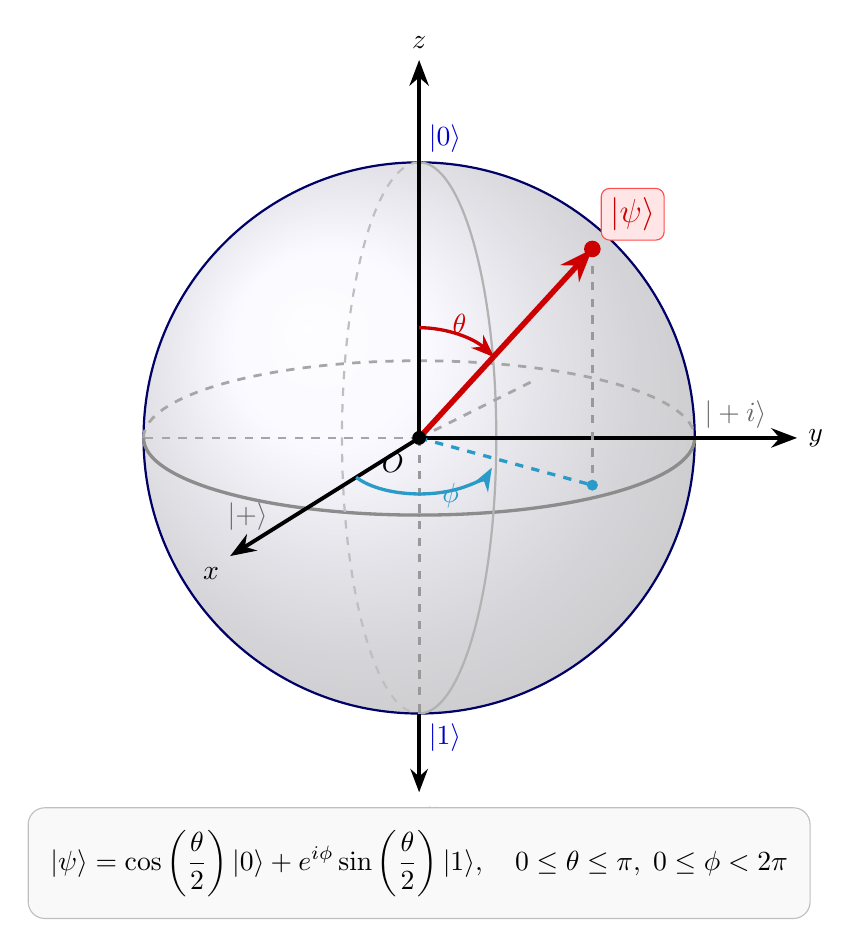
\begin{tikzpicture}[x=1cm, y=1cm, >=Stealth]

  % Coordinates
  \coordinate (O) at (0, 0);
  \def\R{3.5}

  % Background sphere shading
  \shade[ball color=blue!10, opacity=0.3] (O) circle (\R);
  \draw[thick, color=blue!40!black] (O) circle (\R);

  % Equator (XY Plane)
  \draw[dashed, color=gray!70, line width=1pt] (-\R, 0) arc (180:0:{\R} and {0.28*\R});
  \draw[thick, color=gray!90, line width=1.2pt] (-\R, 0) arc (180:360:{\R} and {0.28*\R});

  % Meridian (YZ Plane)
  \draw[dashed, color=gray!50, line width=0.8pt] (0, \R) arc (90:270:{0.28*\R} and {\R});
  \draw[color=gray!60, line width=0.8pt] (0, -\R) arc (-90:90:{0.28*\R} and {\R});

  % Axes
  % -z axis
  \draw[dashed, gray!80, line width=1pt] (0, 0) -- (0, -\R);
  \draw[->, thick, line width=1.2pt] (0, -\R) -- (0, -4.5) node[below] {$-z$};
  \node[blue!80!black, below right] at (0, -\R) {$|1\rangle$};

  % -y axis
  \draw[dashed, gray!70, line width=1pt] (0, 0) -- (-\R, 0);

  % -x axis (into screen)
  \draw[dashed, gray!70, line width=1pt] (0, 0) -- (1.5, 0.75);

  % +x axis (front-left)
  \draw[->, thick, line width=1.4pt] (0, 0) -- (-2.4, -1.5) node[below left] {$x$};
  \node[gray!80!black, left] at (-1.8, -1.0) {$|+\rangle$};

  % +y axis (right)
  \draw[->, thick, line width=1.4pt] (0, 0) -- (4.8, 0) node[right] {$y$};
  \node[gray!80!black, above right] at (\R, 0) {$|+i\rangle$};

  % +z axis (up)
  \draw[->, thick, line width=1.4pt] (0, 0) -- (0, 4.8) node[above] {$z$};
  \node[blue!80!black, above right] at (0, \R) {$|0\rangle$};

  % Quantum State Vector |psi>
  % theta = 50 deg, phi = 42 deg
  \coordinate (P) at (2.2, 2.4);
  \coordinate (Pxy) at (2.2, -0.6);

  % Projections
  \draw[dashed, gray!80, line width=1pt] (P) -- (Pxy);
  \draw[dashed, cyan!80!black, line width=1.2pt] (O) -- (Pxy);
  \fill[cyan!80!black] (Pxy) circle (2pt);

  % Angle phi arc (in xy plane)
  \draw[->, cyan!80!black, line width=1.2pt] (-0.8, -0.5) arc (-148:-15:0.95 and 0.45);
  \node[cyan!80!black, below] at (0.4, -0.45) {$\phi$};

  % Angle theta arc
  \draw[->, red!80!black, line width=1.2pt] (0, 1.4) arc (90:47:1.4);
  \node[red!80!black, above right] at (0.3, 1.2) {$\theta$};

  % State vector arrow
  \draw[->, red!80!black, line width=2pt] (O) -- (P);
  \fill[black] (O) circle (2.5pt) node[below left=2pt] {$O$};
  \fill[red!80!black] (P) circle (3pt);
  \node[draw=red!70, fill=red!10, rounded corners=3pt, font=\bfseries\large, text=red!80!black, above right=3pt] at (P) {$|\psi\rangle$};

  % Formula card at bottom
  \node[draw=gray!50, fill=gray!5, rounded corners=6pt, inner sep=8pt] at (0, -5.4) {
    $|\psi\rangle = \cos\left(\dfrac{\theta}{2}\right)|0\rangle + e^{i\phi}\sin\left(\dfrac{\theta}{2}\right)|1\rangle, \quad 0 \le \theta \le \pi, \; 0 \le \phi < 2\pi$
  };

\end{tikzpicture}
\end{document}
